\section{Compiler}
\label{sec:implementation_compiler}
The compiler consists of multiple classes and stages that work together to compile and optimize the given program. In the following implementation chapter we use specific language when talking about different compilation stages. Any step that is executed in our compiler happens at compile time. The first steps are the analysis, including the lexical, syntactic, and semantic analysis. These are followed by the code generation. Any computations performed in this step are executed at generation time. Lastly, the code is optimized. 
Despite the discrete stages, there are multiple overarching classes and commonly used structures that do not belong to a certain stage. In the following section, we discuss the implementation of general functionalities and introduce the commonly used structures.

When the compiler program is started, the main function calls the Command Line Interface class to parse the arguments to the compiler data class. The compiler data is used to enable and control the compilation process; it contains all required information, such as the path to the input and output files. Furthermore, it specifies which optimizations are to be applied to the compiled program. Lastly, it indicates whether the compilation process is to be executed verbosely. 

After the compiler data is parsed, the main function passes it to the compile function of the compiler class. This is a static class containing general compilation and printing functionalities as well as corresponding properties. We implement it as a static class so that all parts of the program can easily access its functions and properties. The first property of the compiler is the \texttt{Printer} function; its default value is the native console printing function of C\#, but it can be set to any arbitrary function that takes a string as an input and does not return anything. While this property is not changed in a normal compilation process, it is used to check the console output of the compiler in the test cases. Secondly, the verbose property indicates whether the compiler prints not only the errors to the user but also the warnings and informational logs.

To interact with the printer property of the compiler, there are a variety of different printing and logging functions; in the end, all use a single print function that uses the printer property to display a given message. While the printing functions, used for printing errors and warnings, call the print function directly, the logging functions have an additional check so that they only print if the compiler is executed verbosely. Lastly, the logging functions also use compiler services of the runtime to allow for special injections. All of the logging functions have the optional member name and line number arguments that are annotated with a special attribute. In turn, if the optional arguments are not set, the compiler injects the name of the caller for this function as well as the line number where it was called. This can be helpful when trying to debug issues with the compiler.

The compile function handles the entire remaining compilation process. First, it retrieves the program code from the given input path. For the reading and saving of files, a separate \texttt{IOHandler} class exists that has some basic logic for reading and writing files. Then, the parse tree is created and passed to the semantic analysis of the compiler. Here, all errors and warnings are printed to the user. If any errors are thrown, the compilation is aborted. Next, the code is generated from the parse tree. If the compilation resulted in an error, again, the compilation is aborted. After the code is generated, it is optimized based on the optimizations given in the compiler data. Lastly, the resulting program is written to the file specified by the output path.

\subsection{Command Line Interface}
\label{sec:implementation_cli}
As the interface between the programmer and the compiler itself, the command line interface (CLI) is an essential part of the compiler. 
Its purpose is to interact with the programmer and create the compiler data, which specifies the behavior of the compiler. 
To achieve this, the CLI consists of two different parts. The first are the attributes that are used to annotate the compiler data class, and the second part is the CLI handler; it parses the input arguments and creates the compiler data from them. Additionally, it prints the help text to the console if needed.

An attribute is a C\# class that can be used to annotate fields and properties of another class; together with reflection, it can be used to create a modular and easily extendable compiler data class with parameters and descriptions for each compiler data property. Reflection allows programs to get information on types of loaded assemblies. In our case, we are interested in the information on classes, more specifically information on properties of the compiler data class. We create custom attributes with a class that inherits from the \texttt{Attribute} class and contains the required information about the properties we need. With reflection, our program can get a list of all properties with specific attributes and use their information to create, \eg, the help text of the CLI. In turn, we have two custom attributes in our program. The first is the \texttt{CLIParameterAttribute}, which specifies both the short and long name of an attribute corresponding to the compiler data property. For example, in the case of the input path property, the short name is a lower case ``i'' and the long name is ``input''. The second attribute is the \texttt{CLIDescriptionAttribute}; it contains a description for the property it is applied to. Then, this description can be displayed in the help text. In the case of the input path property, the description describes that the parameter describes the path to the input file. The code for the input path property example is depicted in Fig.~\ref{fig:implementation_inputPathAttribute}.

\begin{figure}[htp]
    \centering
    \begin{lstlisting}[style=CSharp]
[CLIParameter('i', "input")]
[CLIDescription("Path to the input file.")]
public string InputPath { get; set; } = string.Empty;
    \end{lstlisting}
    \caption{The input path property declaration with its parameter and description attribute.}
    \label{fig:implementation_inputPathAttribute}
\end{figure}

To parse the command line arguments and create the compiler data from it, the command line interface class is used; it consists of functions to parse the arguments and print the help text to the console. Since the syntax for the CLI argument input is very basic, the command line parsing itself is basic. The input string is split at each space and given to the function as a string array. First, the function retrieves the CLI parameter attributes for all compiler data properties. Then, it iterates over the string array and, for each array entry, checks whether the parameter attribute matches the string; for example, in the case of the input path property, the string would have to be either ``-i'' or ``--input''. If this is the case, the corresponding parsing function, depending on the matched argument, is called with the string array and a reference to the current index. A reference to the index is used to allow for further changes to the index, depending on the number of possible arguments for a parameter. For example, the verbose parameter will always return true and not change the index, while a path parameter will increment the index and return the next string of the array. If no attribute can be matched or an argument exception is thrown in the process, the compiler will notify the user of the invalid or missing argument and print the help text to clarify the compiler options.

The help text is created based on the attributes of the properties in the compiler data class. Firstly, the function retrieves both the parameter and description attributes. Since the compiler data class does not include the help parameter, as it is only used in the CLI context, the help text manually prints its information. Then, the parameters are iterated. For each parameter, a matching description is searched. If no description can be found, the text defaults to a message indicating that none is available. Lastly, both the parameter and corresponding description are printed to the console.

\subsection{Symbols}
\label{sec:implementation_symbols}
The symbols are a major part that is used in most stages of the compilation process, mainly the semantic analysis and code generation; they are used to store all necessary information on data type, composite gates, and similar objects in the language. The basis is an abstract symbol class that consists of an identifier and error context property. The identifier uniquely identifies a symbol in the scope it is used while the error context saves information about the symbol and its declaration environment to be used for possible error messages. In total there are eight different symbols that are derived from the class. In the following, we discuss these symbols and how they are used in the compiler. The hierarchy of the symbol classes is depicted in the diagram in Fig.~\ref{fig:implementation_uml_symbols}.

\begin{figure}[htp]
    \centering
    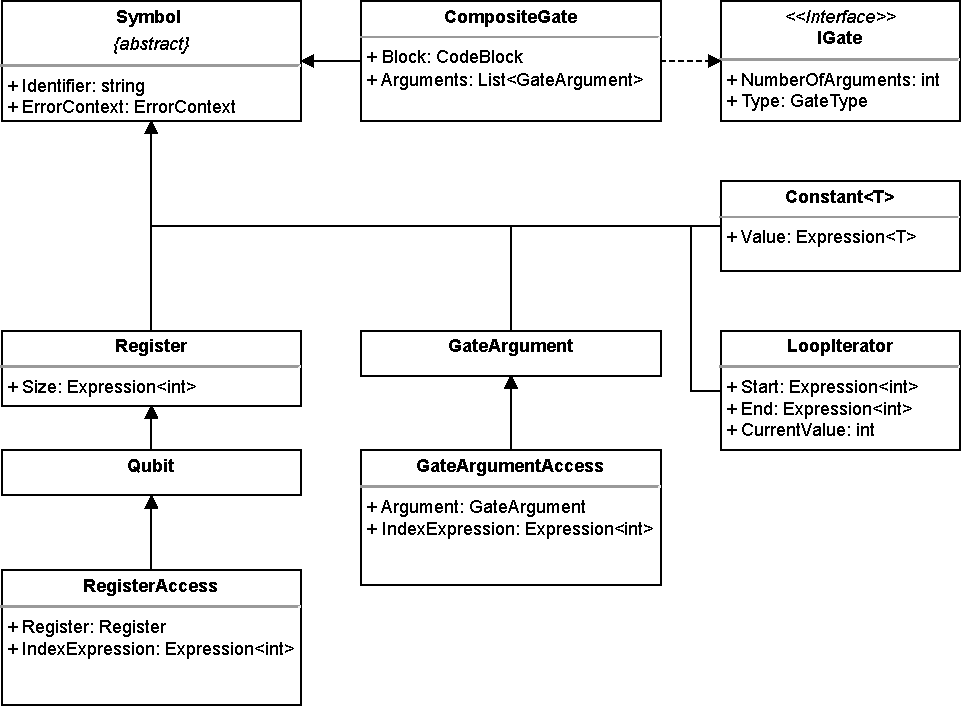
\includegraphics[width=.9\textwidth]{../figures/drawio/uml_symbols.pdf}
    \caption{A diagram showing the hierarchy of symbol classes.}
    \label{fig:implementation_uml_symbols}
\end{figure}

There are three different symbols for quantum data types. The first kind is the register. Furthermore, it is the basis of all other quantum data type symbols. Besides the inherited properties, it consists of an expression that represents the size of the register. The expression specifying the size of the register may not be evaluable when its symbols are created because the value of some identifiers may be known only at generation time.
For example, the body of a loop statement is unrolled at generation time, and the value of the loop iterator depends on this iteration. In turn, the value of the iterator identifier may not be known when the register symbol is created. Therefore, instead of saving a constant value, the symbol specifies the expression for its size. Then, when the code is generated and all values are known, the expression can be evaluated.

Next, the qubit symbol inherits from the register. While physically the qubit is the basic element and a register consists of qubits, in our case, it is useful to assume that a qubit is a special case of a register where the size is one so that the qubit can inherit the register symbol properties and functions. Furthermore, instead of differentiating between a qubit and register declaration, a register declaration is sufficient for this hierarchy, only requiring a differentiation when printing the code. In turn, all registers with size one are inherently optimized to be qubits in the target code. Besides setting the size to one, the qubit symbol has no additional attributes.

The last quantum data type symbol is the register access. This symbol is necessary because the access of a register is not implemented as an expression. Since a register access cannot be used in any expression and only in the context of a gate application or if-statement, instead of implementing special quantum expressions that can only be used in limited cases, we create another symbol. The register access symbol inherits from the qubit symbol, as it can be used whenever a qubit symbol can be used. For example, in the case of a gate application statement, a list of qubits, to which the gate is applied, is saved. In turn, since each register access is a qubit, no additional list or differentiation is required for the gate application, only a virtual function to return the translated qubit code. The symbol also contains an integer expression that specifies which index is accessed and the register that is accessed. Similar to the size expression of the register symbol, the expression is saved since it may not be evaluable when the symbol is created.

There are two symbols for classical data; these are the constant symbol and the loop iterator. The constant symbol represents a named constant of differing types. To allow for different variable types, the symbol has a generic parameter \texttt{T}. Additionally, the generic parameter is restricted to implementing the number interface, indicating that it is a numeric type. Furthermore, as with the other symbols where a property may depend on a value that is not known at the time of creation, the constant symbol value is given by an expression. This expression is of the type \texttt{T}.

Secondly, the loop iterator symbol is the other symbol used to represent classical data; however, it is specifically designed for the loop statement of our language and its special properties. It is used to unroll the loop body and propagate the value of the current iteration of the loop. To achieve this, the symbol contains the start and end indices as integer expressions; they can be evaluated when the code is being generated. Furthermore, the symbol contains a current value property that contains the value of the current iteration. When the code for the loop body is unrolled by being iterated, any reference to the iterator symbol will evaluate to the current value.

The last three symbols are all related to the composite gates. Firstly, there is the composite gate symbol itself. It is created when a composite gate is declared and, later on, is used whenever it is referenced in a gate application statement. To allow for a predefined gate, an interface is declared that represents the important attributes of a gate; these are the number of arguments to the gate and the gate type. The gate type differentiates between the different predefined gates, such as the Hadamard or $X$ gate, and the composite gates. This gate interface is implemented by the composite gate. Besides the properties required by the gate interface, the composite gate symbol consists of a block property and an arguments property. The block property contains the code block that is the body of the composite gate; it is used to inline the statements of the gate whenever it is applied. Secondly, the arguments are a list of gate argument symbols that represent the arguments that can be passed to the composite gate.

The second kind of composite gate-related symbols are the above-mentioned gate argument and gate argument access symbols. Both represent an argument to a composite gate and serve as a placeholder for the symbol of the argument that is passed when the gate is applied. When inlining, the placeholder, \ie, the argument symbol, is mapped to the given argument. Furthermore, while the composite gates themselves can only operate on the previously discussed quantum data type symbols, the programmer does not specify the type of the argument, which can be both a qubit or quantum register, when declaring the composite gate. Therefore, we introduce a symbol that will ignore type checking until the composite gate is called and the arguments are specified. Then, if an argument is of an invalid type for a specific use, a type error is thrown. Similar to the register access, an additional gate argument access symbol is required because an access cannot be represented as an expression; it inherits from the gate argument symbol, has a reference to the gate argument that is accessed, and an integer expression that evaluates to the access index at generation time.

\subsection{Symbol Table}
\label{sec:implementation_symbolTable}
The symbol table is a data structure that saves all symbol information and offers functions for adding new symbols and retrieving symbol information. For example, a new symbol can be added with the \texttt{AddSymbol} function, and symbol information can be obtained based on the identifier with the \texttt{GetSymbolInfo} function.

To allow for different symbol contexts, the scope data structure is used. Scopes are used to enable the declaration of different variables with the same identifier in independent scopes, \ie, two scopes where neither is the other's ancestor nor descendent. The scope class contains an identifier dictionary that maps a string, in this case representing the identifier, to the corresponding symbol. Because of the quantum if-statement, a scope can also be guarded by a qubit. Therefore, a scope has an optional guard symbol that either references the symbol that guards the scope and all descendants or is null. Lastly, the scope contains a reference to the code block it belongs to. While the parse tree is traversed, each statement is added to the code block of the current scope. Later, the code block can be passed along in the generation to, \eg, create the loop statement belonging to the scope.

The scopes are saved in the symbol on a stack. Each time a new code block is entered when traversing the parse tree, a new scope is pushed onto the scope stack. Similarly, each time a block is exited, the scope stack is popped to remove the latest scope from the data structure. To simplify the interactions with the scope stack, the symbol table contains both a current scope and a current identifier map property; both reference the top-most scope on the stack and the identifier map of the current scope, respectively.

While the scope data structure holds a reference to the guard symbol, the symbol is known before the creation of the current scope because first the if-statement is traversed, then the code block. Therefore, the class interacting with the symbol table would need to save the current identifier and pass it to the push scope function. To avoid this additional complexity, the symbol table holds a guard stack that can be interacted with by using the additional \texttt{PushGuard} and \texttt{PopGuard} functions. In turn, the symbol table can use the scope stack to pass the current guard to a newly created scope. Additionally, guards and scopes are abstracted when using the symbol table such that the class traversing the parse tree only needs to push and pop the correct information and is not required to save the current guard information.

Lastly, the symbol table contains a property that generates a unique identifier. To achieve this, it contains a private integer field \texttt{\_uniqueId} that is initialized with a value of zero. Each time the unique identifier property is retrieved, the id is incremented. The identifier is just the id with a ``id\_'' prefix. The property is used when generating the OpenQASM code, as it does not allow for different variables with the same identifier. While this is a very simplistic approach, these resulting identifiers are always unique, as long as the same symbol table is used, and the resulting identifiers are predictable. This predictability is especially helpful when creating test cases for the translation of source code, as we can simply give the expected target code.

\subsection{Error Handling}
\label{sec:implementation_compiler_errorHandling}
Error handling is an essential part of both the semantic analysis and code generation phase of the compiler; without clear and informative error messages, debugging compilation errors is both challenging and tedious. 
Therefore, our compiler supports a number of different errors and exceptions, mainly differentiating between two types of errors with different severities. The first type is the \emph{warning}. A warning from the compiler can indicate issues in the source code that may cause unintended behavior. However, the issue itself does not prevent the compilation of the program and is simply an indication that there may be something wrong. In contrast, the \emph{critical error} is caused by a flaw in the source program that prevents the correct compilation and will result in the abortion of the compilation. In the following, we will discuss the error handling of our compiler in general, different warnings and critical errors the compiler may raise, their corresponding causes, and implementations.

Any compilation error caused by the user is represented by the abstract compilation error class, which contains three different properties. The first property is the error type; it indicates the severity of the error, as described above. Secondly, the description property should hold a description of the error that can be used to inform the programmer what issue occurred. Lastly, the error context saves relevant information about the source code properties of the error; it is implemented as a \texttt{struct} that contains both the line and column index of the source code location of the error. The error context can be created either from the line and column directly, the token where the error occurred, or the parsing rule with which the error is associated. In many cases, the error context can be created when the error occurs. For example, if an undefined identifier error is found in the declaration analysis, the parser rule context is given, and the error can easily be created from it. However, in other cases, errors may be thrown at generation time, and the corresponding parser rule context may no longer be known. Therefore, all symbols also contain the error context corresponding to their declaration.

While the abstract compilation error class contains general properties that are required for all errors, each error may contain additional properties that are required to give a clear and informative description of the error. Additionally, since many errors occur in reference to a specific identifier, the compiler uses an additional abstract identifier error that contains a string property that holds the identifier. In the following, we will go through the warnings and errors. All of their classes, including their respective properties, are depicted in Fig.~\ref{fig:implementation_uml_errors}.

\begin{figure}[htp]
    \centering
    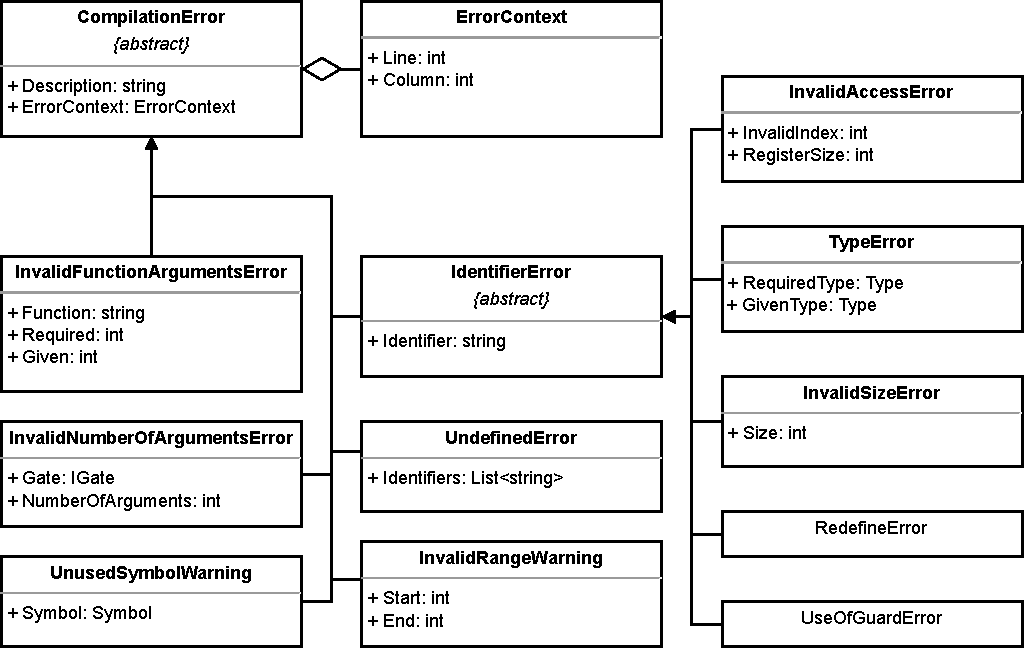
\includegraphics[width=.9\textwidth]{../figures/drawio/uml_errors.pdf}
    \caption{A diagram showing the hierarchy of error classes.}
    \label{fig:implementation_uml_errors}
\end{figure}

The compiler can throw two different kinds of warnings. The first is the invalid range warning; it can occur in the context of loop statements. The loop statement iterates over a range that is defined by the user. It can be given as either a size $n$ and iterate from zero to $n-1$ or a start and end index, $i_{Start}$ and $i_{End}$, respectively, and iterate from the start to the end. However, the range iterator is designed to only increase. Therefore, a range where $i_{Start} \geq i_{End}$ is invalid. Since the loop statement is unrolled at compile time, a range with a size less than or equal to zero can just be ignored. However, the user may not intend this behavior. Therefore, the compiler warns the user that the range is invalid. The class for the warning contains the start and end indices for the invalid range.

Secondly, the unused symbol warning is raised when a symbol, \eg, a register or composite gate, is defined in the source code but never used. This symbol is stored in the corresponding error class. The unused symbol does not have any negative effect on the compilation, and the optimization step can easily remove, \eg, an unused register. Therefore, this is only a warning, and the program can be compiled. However, an unused symbol may indicate that the wrong symbol was used somewhere else or part of the program is no longer used. Hence, the user is warned of the unused symbol, and unintended behavior may be prevented.

The first critical error is the invalid access error. It occurs when a register is accessed at an invalid index $i$, \ie, $i$ is either smaller than zero or larger than $size - 1$, where $size$ is the size of the register. While this error could easily be ignored and would cause no issue when compiling the program, the resulting code would be an invalid circuit description. The invalid access error saves the identifier that is accessed, inheriting from the identifier error, as well as the invalid access index.

Secondly, the invalid number of arguments error for gates and functions is caused when the number of arguments given to either a gate or function does not correspond to the number of required arguments. For example, the Hadamard gate always expects one argument, while the controlled-not gate requires two. Similarly, the \texttt{sizeof} function operates on only one argument. The compiler cannot proceed when given too few arguments; for the opposite case, while dropping any leftover arguments is possible, it would result in unexpected behavior.
Therefore, the compiler reports an error for both cases and aborts the compilation. In the case of the invalid function argument error, the function as well as the number of required and given arguments are saved; for the gate error, the given number of arguments and the gate interface object, containing both the gate type and number of required arguments, are saved.

Another error is the invalid size error. It occurs when a register is declared with an invalid size. A size is invalid if it is less than or equal to zero. A register with no entries cannot be used for anything and likely indicates an issue in the program, while a register with a negative amount of entries is impossible. Therefore the compilation is aborted and the error is thrown. In the corresponding error class, which inherits from the identifier error, the invalid size is saved as well as the identifier used in the declaration.

The next two errors are concerned with the declaration of variables in a given context; they are the undeclared and already-declared errors. An undeclared error is raised when a variable is used in a context where it is not defined. In this case, the symbol table does not have a symbol stored for the given identifier, and the compiler cannot continue. In contrast, the already-declared error occurs when a variable is declared in a context where the same variable identifier has already been assigned to a different symbol. While the compiler could overwrite the previous declaration, this can easily lead to unexpected behavior, and, in turn, we do not allow a declaration in the same scope to be overwritten. While the redefine error saves the identifier that is redefined, inheriting from the identifier error class, the undefined error saves a list of possible undefined identifiers. A list of identifiers is saved because, in our implementation, an expression returns a list of undefined identifiers, which is used to create the error.

The type error is thrown when a variable is used in a function or gate but is not the required type. Languages with loose typing may be able to convert some types to the required type by, for example, parsing the integer value of a string. However, this can not only result in unexpected behavior and hard-to-debug errors in the code, but, in the case of a quantum language, it may also require the conversion between classical and quantum data, which is not easily achievable. In this case, the error class inherits from the identifier error class and contains the required and given type as well as the identifier of the symbol.

Next, another error is the use-of-guard error; it occurs when a qubit is referenced in a context that is guarded by itself. While the compiler can easily translate any such occurrence, they result in an invalid circuit description. As described in Sec.~\ref{sec:background_branching}, a gate that operates on and is controlled by the same qubit cannot be reversible. Therefore, the compiler prevents the generation of an invalid circuit and aborts the compilation. The error class only contains the corresponding identifier and, in turn, inherits from the identifier error.

Finally, the last error is the invalid declaration error. Since composite gates are only meant to operate on the registers and qubits given as arguments, our language does not allow for register or qubit declaration in the context of a composite gate. Any register or qubit declaration inside the scope of a composite gate declaration will result in an invalid declaration context error. The error class inherits from the identifier error class and, in turn, contains the identifier of the corresponding invalid declaration. 

One advantage of a semantic analysis separate from the code generation is that, if an error is found, the semantic analysis can continue. For example, if an undefined identifier error occurs while generating code, the code generation can no longer continue as the identifier cannot be mapped to a symbol, and, therefore, the information for the code generation is incomplete. However, a semantic analysis can continue as it does not need any more information about a symbol than its existence. In turn, while errors in the code generation phase use typical error handling with exceptions that abort the tree traversal, the semantic analysis uses a custom error handler. Mainly, this error handler object consists of a list of compilation errors and a report function that takes an error and adds it to the list. Additionally, the handler also contains properties that indicate whether it contains critical errors and two lists that return only the critical errors or warnings, respectively. After the semantic analysis, the compiler will iterate over the errors in the handler and print them as either errors or warnings, depending on their error type.

Besides the code generation exception, there exists the internal exception. This exception is used in all stages of the compiler. The code generation exception wraps compilation errors in the code generation stage where the user is at fault. However, there may be cases where the compiler enters an error state for which the user is not responsible, \eg, an unexpected null reference. For these cases, the internal exception is used.